\subsubsection{8.12.15}
Today we discussed results of competition and improvements that we should make in the robot\newline
Problems and solutions for each module:
\begin{enumerate}
	\item Wheel base:
	\begin{table}[H]
		\vspace{-2mm}
		\begin{center}
			\begin{tabular}{|p{0.15\linewidth}|p{0.4\linewidth}|p{0.55\linewidth}}
				\hline
				Problem & Solution\\
				\hline
				Can't climb to mountain  & To move front wheels forward   \\	
				\hline
				Chain isn't protected & Install protection of plexiglass or metal\\
				\hline
			\end{tabular}
		\end{center}
	\end{table}
	\item Lift and bucket:
	\begin{table}[H]
		\vspace{-2mm}
		\begin{center}
			\begin{tabular}{|p{0.15\linewidth}|p{0.4\linewidth}|p{0.55\linewidth}}
				\hline
				Problem & Solution\\
				\hline
				Bucket don't turn to side  & To make mechanism that turn bucket to side   \\	
				\hline
				Lift can't reach high box from low zone & To make mechanism that extend moving beam of the lift\\
				\hline
				Reducer of the motor that move lift broke & To fix axis of the motor more rigidly\\
				\hline
			\end{tabular}
		\end{center}
	\end{table}
	\item Gripper for debris
	\begin{table}[H]
		\vspace{-2mm}
		\begin{center}
			\begin{tabular}{|p{0.15\linewidth}|p{0.4\linewidth}|p{0.55\linewidth}}
				\hline
				Problem & Solution\\
				\hline
				Rotates too slow  & To install transmission with gear ratio 1:2   \\	
				\hline
			\end{tabular}
		\end{center}
	\end{table}
	
	\item Mechanism for scoring climbers 
	\begin{table}[H]
		\vspace{-2mm}
		\begin{center}
			\begin{tabular}{|p{0.15\linewidth}|p{0.4\linewidth}|p{0.55\linewidth}}
				\hline
				Problem & Solution\\
				\hline
				Climbers sometimes get stuck in bucket  & To extend bucket or make it narrower and put climbers on each other  \\	
				\hline
			\end{tabular}
		\end{center}
	\end{table}
	
	\item Also we need to improve programme of aotonomous period. It was decided to turn with help of gyro or compass sensor.
	
	\item In addition during one match NXT brick fell off. So we need fix it more reliable.
	
\end{enumerate}
\begin{itemize}
\subsubsection{9.12.15}

	\item It was estimated place for front wheels.
	
	\item It was started designing of mechanism that turn bucket to side. 

\subsubsection{10.12.15}

	\item It was finished designing mechanism for turning bucket for debris to side.
	
	\item Bucket on F-shaped beam was extended. So climbers don't fet stuck in it.
\subsubsection{12.12.15}
	\item Front wheels were moved forward.
	
	\item Mechanism for turning bucket to side was assembled but servo that move it wasn't installed.
	\begin{figure}[H]
		\begin{minipage}[h]{0.45\linewidth}
			{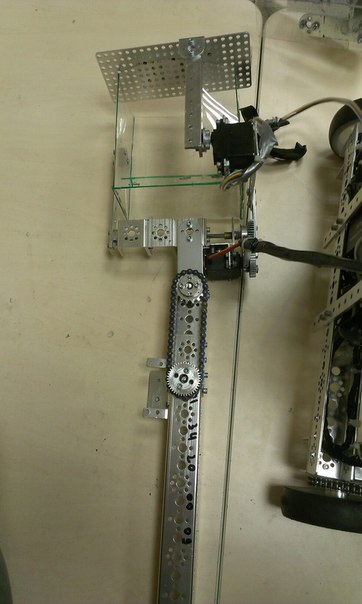
\includegraphics[scale=0.45]{days_L/Meetings/images/09}}
		\end{minipage}
		\hfill
		\begin{minipage}[h]{0.5\linewidth}
			{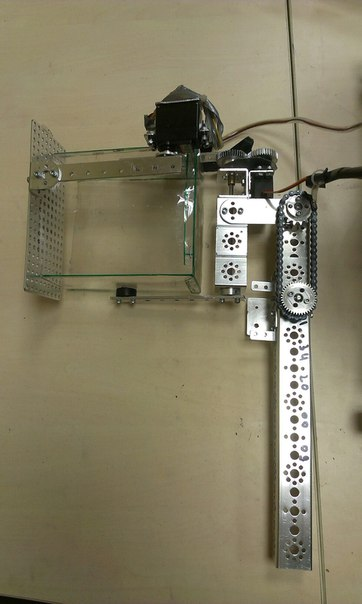
\includegraphics[scale=0.5]{days_L/Meetings/images/10}}
			\caption{Mechanism for turning bucket to side}
		\end{minipage}
	\end{figure}
	
	\item It was started assembling new gripper for debris.
	
\subsubsection{14.12.15}
	\item Climbing to mountain was tested. Robot can reach low zone. It was decided install Lego caterpillars for better traction. After that robot was able to climb to low zone and overcome bottom obstacle by the back wheels. Also it was found that if we move central wheels forward so that back wheels touch second obstacle before central wheels toch first obstacle (now central wheels touch bottom obstacle first) robot most likely will be able to climb to middle zone.
	
	\item It was started installing new gripper for debris.
	
\subsubsection{15.12.15}
	\item It was installed servo that turn bucket to side.
	
	\item The axis of the motor that move lift was fixed rigidly.
	
	\item It was installed protection for chains.
	
\subsubsection{16.12.15}
	\item It was held wiring for servos that turn bucket.
	
	\item The gripper for debris was installed.
\end{itemize}

\fillpage